% $HeadURL$

%%%%%%%%%%%%%%%%%%%%%%%%%%%%%%%%%%%%%%%%%%%%%%%%%%%%%%%%%%%%%%%%%%%%%%
%%%%                   Complex
%%%%%%%%%%%%%%%%%%%%%%%%%%%%%%%%%%%%%%%%%%%%%%%%%%%%%%%%%%%%%%%%%%%%%%

\paragraph{Complex}\label{sec:complex}

A complex glyph represents a biochemical entity composed of other
biochemical entities, whether macromolecules, simple chemicals,
multimers, or other complexes. The composition of a complex can also
be shown using subunits decorators (see below), but these are optional
and it is also correct to show a complex without any subunits. The
complex can be represented by a monomeric glyph (\glyph{Complex monomer}) and a multimeric glyph (\glyph{Complex multimer}).

\begin{glyphDescription}
\begin{glyphIdentity}
  \item owning compartment
  \item name \textbf{or} names of the subunits 
  \item cardinality
  \item The set of state values associated with the subunit decorators
    and the set of state values associated with the Complex.
  \end{glyphIdentity}
\glyphRules
\begin{itemize}
  \item The mutimer glyph must be used if cardinality is greater than
    1.
  \item If no subunits are defined then the complex must have a name.
  \item The subunits of a complex are not EPNs. The complex itself
    represents the pool of entities.
\end{itemize}
\end{glyphDescription}


\subparagraph{\glyph{Complex Monomer}}

This glyph represents a monomeric complex EPN.

\begin{glyphDescription}

\glyphSboTerm SBO:0000253 ! non-covalent complex

\glyphContainer A \glyph{complex} possesses its own container box surrounding the juxtaposed container boxes of its components.  This container box is a rectangle with cut-corners (an octagonal box with sides of two different lengths).  The size of the cut-corners are adjusted so that there is no overlap between the container and the components.  The container boxes of the components must not overlap.

\glyphLabel The identification of a \glyph{named complex} is carried by an unbordered box containing a string of characters.  The characters may be distributed on several lines to improve readability, although this is not mandatory.  The label box has to be attached to the midway between the border of the complex's container box and the border of the components' container boxes.

\glyphAux A \glyph{complex} can carry state variables (see \sect{stateVariable}).  The state of a complex is defined by the set of the all its state variable and all the state variables of all its components.  A \glyph{complex} can also carry one or several \glyph{units of information} (see \sect{unitInfo}). A \glyph{complex} may carry a \glyph{clone marker} (see \sect{cloneMarker}).

\glyphCloning Labeled Clone Marker

\end{glyphDescription}


\begin{figure}[H]
  \centering
  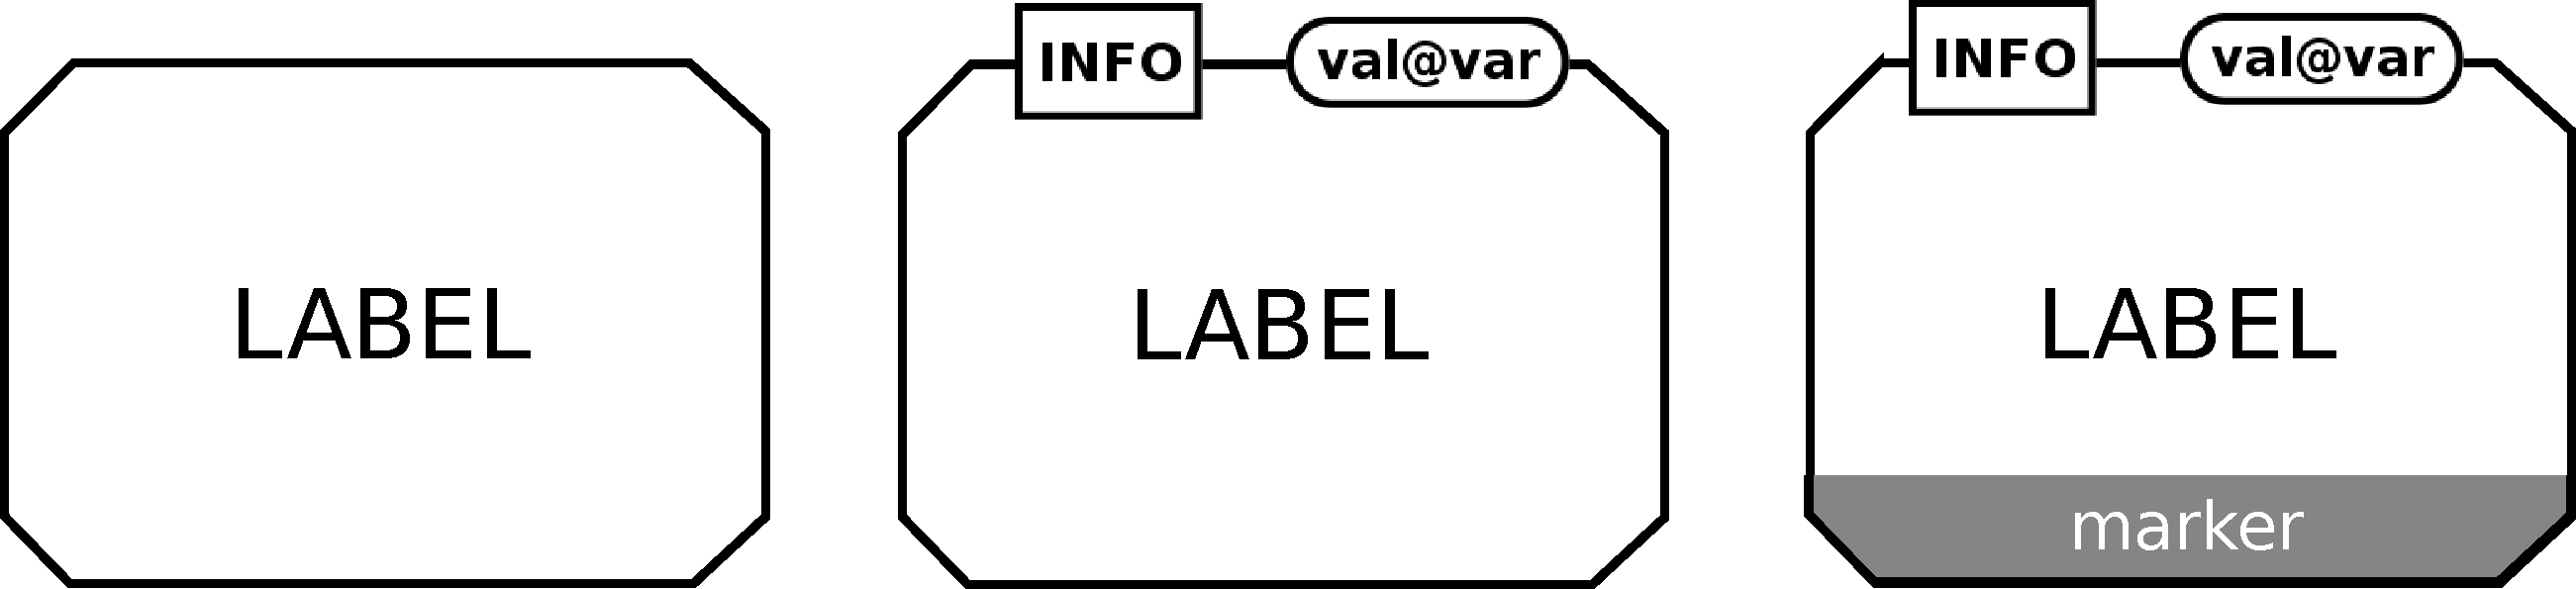
\includegraphics[width=3.5in]{images/complexGlyph}
  \caption{The \glyph{complex} glyph.}
  \label{fig:complex}
\end{figure}

\subparagraph{\glyph{Complex Multimer}}

This glyph represents a multimeric complex EPN.

\begin{glyphDescription}

\glyphSboTerm SBO:0000418 ! multimer of complexes

\glyphContainer A \glyph{Complex Multimer} is represented by two
identical \glyph{Complex} containers shifted horizontally and
vertically and stacked one on top of the other.  \fig{complexMultimer}
illustrates the glyph.

\glyphLabel As monomer.

\glyphAux As monomer.

\glyphCloning Labeled Clone Marker

\end{glyphDescription}


\begin{figure}[H]
  \centering
  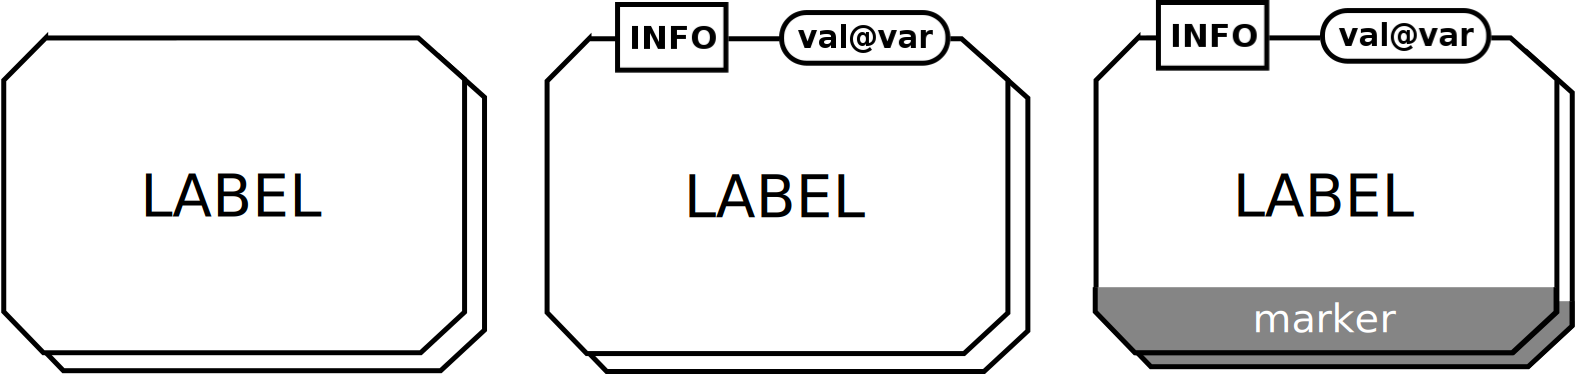
\includegraphics[width = 3.5in]{images/complexMultimerGlyph}
  \caption{The \glyph{Complex Multimer} glyph.}
  \label{fig:complexMultimer}
\end{figure}

\subparagraph{Subunits}

A complex can optionally be decorated with subunit symbols to describe
the composition of the complex. The symbols available are equivalent
to those used by the EPN glyphs including the
\glyph{complex}. Therefore it is possible to describe complexes within
complexes. Subunits may contain labels. The following rules apply to
the use of subunits in a complex:

\begin{itemize}
\item The subunit can contain any symbol used by an EPN glyph.
\item Subunits that use the \glyph{Complex} glyph can also contain
  subunits. There is no limit on such nesting. The namespace rules
  below apply.
\item Mutimeric glyphs can also be used a subunits. They should
  include the cardinality of the mutimer in the manner spercified for
  the equivalent EPN.
\item Subunits with the same name can be repeated one or more times.
\item Subunits may be assigned one or more state variables. Each state
  variable actually belongs to the Complex.
\item The subunit defines a namespace for its state variables, e.g.\,
  subunit ``A'' assigned a state variable ``P@Ser202''  and a subunit
  ``B'' assigned the same state variable can be distinguised as
  A:P@Ser202 and B:P@Ser202.
\end{itemize}

The example in figure \fig{complexSubunits} illustrates the use of
subunits in a complex shows an equivalent compex without
subunits. This is an import point. For every \glyph{Complex} drawn
with subunits it will always be possible to drawn an equivalent
version that does not use contains subunits.

\begin{figure}[H]
  \centering
  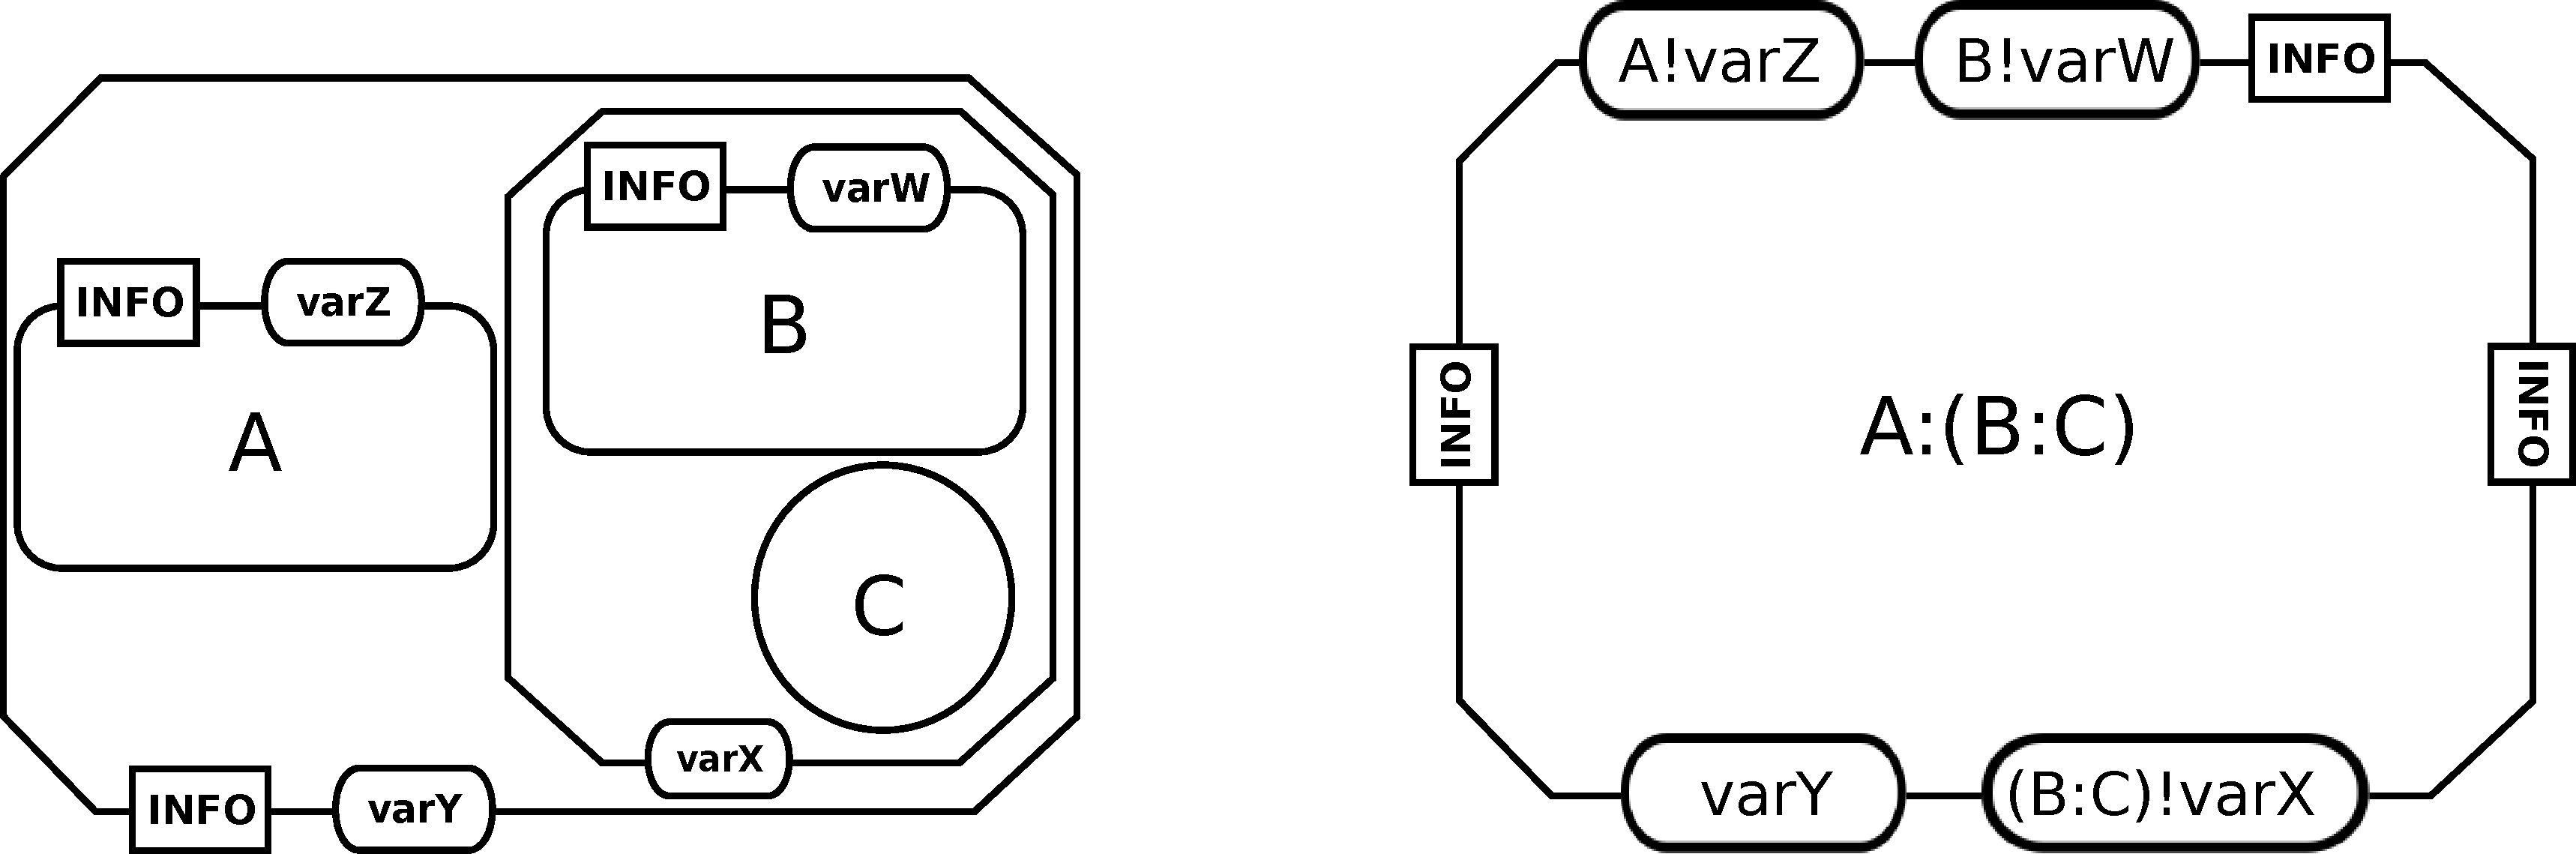
\includegraphics[width = 3.0in]{images/complex}
  \caption{Both these complex glyphs are equivalent. The one on the
    left is described using subunit decorators, the one on the right
    describes the same thing without them.}
  \label{fig:complexSubunits}
\end{figure}

% Show the available glyphs to be used as subunits.


%%%%%%%%%%%%
% Put the following in the semantics section

% \subsubsection{Attributes}


% The complex has the following attributes (those in \emph{italic} identify the complex):

% \begin{description}
% \item[\emph{name}]
% \item[\emph{cardinality}] The number of subunits of the complex. If
%   cardinality $> 1$ then the \glyph{Complex Multimer} must be
%   drawn. Otherwise a \glyph{Complex} is drawn. The cardinality is an
%   integer $>0$.
% \item[\emph{compartment}] The complex must belong to one compartment.
% \item[state variables] The complex can have zero, one or more state
%   variables. 
% \item[clone ID]
% \end{description}


% The following is for [X]Emacs users.  Please leave in place.
% Local Variables:
% TeX-master: "../sbgn_PD-level1"
% End:
